\documentclass[a4paper]{article}

\usepackage{ReportTemplate}

\usepackage{setspace}
\usepackage{amsmath}
\usepackage[hidelinks]{hyperref}

\title{Project 2:Kaldi的安装和基本使用}
\name{邱一航}
\studentid{520030910155}

\begin{document}

\maketitle

\setcounter{section}{-1}
\section{安装环境}
笔者在Windows提供的Linux子系统,即WSL(Windows Subsystem for Linux)环境下安装Kaldi。

所安装的WSL版本为2.0,笔者在该子系统中安装Ubuntu操作系统,Ubuntu版本为Ubuntu 20.04。WSL环境下已预先安装了CUDA 10.1。

%请简要描述安装Kaldi的过程并跑出一个基本的示例程序,记录你在这个过程中的步骤和遇到困难,并简要描述是如何解决的。

%请使用简练准确的语言撰写报告,不要一味追求数量。报告至多4页,多出部分将被忽略。

%\textbf{请在报告写作完成后删除本章。}

\section{Kaldi的安装}
从https://github.com/kaldi-asr/kaldi下载Kaldi源码,解压后根据INSTALL文件的提示逐步操作即可完成Kaldi源码的编译和相关安装。

\subsection{Kaldi源码编译过程}
\subsubsection{$\mathtt{tools}$文件夹内的编译}

首先运行$\mathtt{extras/check\_dependencies.sh}$文件,该文件会检查Kaldi所需要的前置条件是否满足。根据指示安装automake、autoconf等Kaldi所需要的库,并安装Intel MKL。

之后运行$\mathtt{make\ \text{-}j\ 4}$,使用四个CPU核来完成Kaldi所需库的编译。

由$\mathtt{src}$内INSTALL文件可知,这一阶段完成了OpenFst的编译与ATLAS库、CLAPACK库的头文件获取。

\subsubsection{$\mathtt{src}$文件夹内的编译}

运行$\mathtt{./configure\ \text{--}shared}$,为Kaldi的编译即可完成MKL的配置。

之后运行$\mathtt{make\ depend\ \text{-}j\ 4}$和$\mathtt{make\ \text{-}j\ 4}$完成Kaldi源码的编译。



\subsection{遇到的困难}

\subsubsection{包管理器软件包列表更新}

根据$\mathtt{tools/extras/check\_dependencies.sh}$的运行结果进行Kaldi所需库的安装时,安装失败并返回以下错误信息。

\begin{lstlisting}
E: Unable to fetch some archives, maybe run apt-get update or try with --fix-missing?
\end{lstlisting}

    \textbf{解决}:发现是Ubuntu包管理器软件包列表并非最新版导致的。根据提示运行$\mathtt{apt\text{-}get\ update}$后重新进行Kaldi所需库的安装即可。

\subsubsection{WSL管理员权限}
    安装MKL时提示需要管理员权限。
    
    \textbf{解决:}使用以下指令运行$\mathtt{install\_mkl.sh}$。
    
\begin{lstlisting}
sudo extras/install_mkl.sh -sp debian intel-mkl-64bit-2020.0-088
\end{lstlisting}

\subsubsection{MKL配置}
    在$\mathtt{src}$目录下运行$\mathtt{./configure\ \text{--}shared}$进行MKL配置时,提示错误如下。
    
\begin{lstlisting}
***configure failed: CUDA 10_1 does not support c++ (g++-9).
You need g++ < 9.0. ***
\end{lstlisting}

\textbf{解决}:查看WSL环境下g++编译器版本,发现是9.4.0,而CUDA 10.1不支持该版本的g++编译器。笔者尝试下载g++-4.8版本,发现无论使用apt、aptitude、apt-get都返回如下错误。

\begin{lstlisting}
    E: Package 'g++-4.8' has no installation candidate
\end{lstlisting}

大概率是由于Ubuntu 20.04的软件包列表中已经不支持较低版本的g++和gcc编译器。因此笔者转而下载g++-7(7.5.0版本)并将默认编译器切换为g++-7。再次使用$\mathtt{./configure\ \text{--}shared}$进行MKL配置,配置成功。


\subsection{Kaldi的基本结构}
Kaldi编译后的源码的根目录共有8个文件夹,它们的内容分别如下。

\begin{table}[th]
  \setstretch{1.3}
  \centering
    \begin{tabular}{ll}
    \toprule
    目录名 & 内容 \\
    \midrule
    cmake & 使用C++进行源码编译的文件。\\
    egs & 一些Kaldi使用的示例代码。\\
    misc & Kaldi相关的论文及htk脚本。\\
    scripts & 包含了RNNLM的实现和Wakeword。\\
    src & 包含了Kaldi的源码。\\
     & 包含了Kaldi依赖库的安装脚本。\\
    tools& 包括OpenFst、ATLAS、CLAPACK、\\
    & IRSTLM、SRILM等。\\
    windows & 在Windows系统下安装所使用的脚本。\\
    \bottomrule
    \end{tabular}
\end{table}



\section{Kaldi的基本使用}
笔者使用了egs目录下的yesno这一示例来尝试使用Kaldi。

\subsection{示例程序运行中的困难}
直接在对应目录下运行$\mathtt{./run.sh}$,过程中显示了两类错误。

第一类错误是在读取环境变量时发生错误。这里主要是路径中含有空格的问题,而WSL的环境变量默认与Window系统环境变量挂钩,因存在含有空格的路径(如C:/Program Files/)。因此读取环境变量PATH时出错(在空格处自动截断了,读到了“Files”开始的一串字符串)。

\begin{lstlisting}
sh: 1: export: Files/WindowsApps/CanonicalGroupLimited.Ubuntu20.04onWindows_2004.2022.8.0_x64__79rhkp1fndgsc:/mnt/e/Program: bad variable name
--> ERROR: data/lang/L.fst is not olabel sorted
\end{lstlisting}

\textbf{解决}:使用以下指令修改WSL环境下的环境变量\$PATH。(第一行是查看\$PATH的内容,第二行是修改\$PATH。

\begin{lstlisting}
echo \$PATH 
export PATH=home/balthasar/.local/bin:/usr/local/sbin:/usr/local/bin:/usr/sbin:/usr/bin:/sbin:/bin:/usr/games:/usr/local/games:/usr/lib/wsl/
\end{lstlisting}

第二类错误是“未找到对应文件”,错误信息如下。

\begin{lstlisting}
local/prepare_data.sh: line 39: utils/utt2spk_to_spk2utt.pl: No such file or directory
\end{lstlisting}

检查发现utils文件指向另一个目录下的utils文件夹,不知道为什么WSL未能成功实现utils的重定向。

\textbf{解决}:笔者暂时将这类文件都用所指向的文件或文件夹替代,将目标文件和文件夹复制到当前目录下。这样处理后程序确实能正常运行。

两类错误应该都和WSL的系统环境变量\$PATH相关。但笔者暂未找到更好的解决方案。

\subsection{示例程序的基本结构}
由$\mathtt{run.sh}$可知,yesno示例的训练过程如下:

第一阶段是数据下载、预处理与模型准备。从指定源下载waves\_yesno数据集,随后使用$\mathtt{prepare\_data.sh}$和$\mathtt{prepare\_dict.sh}$准备数据和发音字典,用$\mathtt{utils/prepare\_lang.sh}$和$\mathtt{local/prepare\_lm.sh}$准备状态机。

第二阶段是特征提取。从准备好的数据中提取声学特征,作为后续声学模型的输入。该示例中提取了MFCC特征,即梅尔滤波器倒谱系数。

第三阶段是声学模型训练。本示例中训练使用单音素建模的状态机。

第四阶段是解码与效果测试。在测试集上测试训练后的模型的效果,并计算整个测试集上的词错误率(WER)。

\subsection{运行结果展示}

\begin{figure}[htb]
  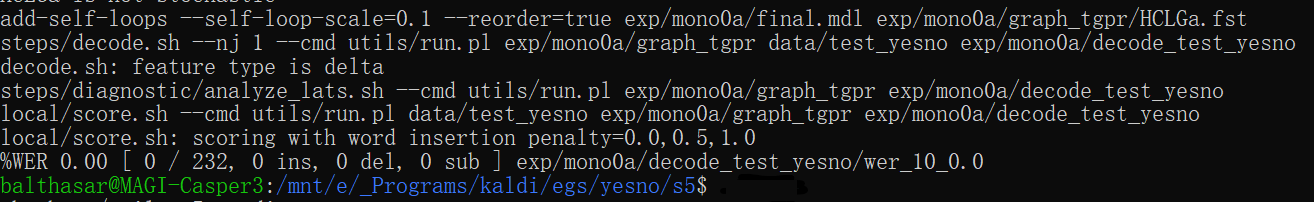
\includegraphics[scale=0.39]{run.png}
  \caption{The Result of $\mathtt{run.sh}$}
  \label{fig1}
\end{figure}

运行run.sh后结果如上图。结果显示WER为0\%,在测试集上准确率很高。

\end{document}